\chapter{Другие оценки}

В ходе исследовательской работы было поставлено также несколько других вычислительных экспериментов. Они не относятся непосредственно к использованию схемы Неймана-Улама, но также представляют собой попытки снизить временную сложность вычисления оценки стоимости Американского опциона.

\section{Анализ распределения состояний с помощью эмпирической функции распределения}
	    \subsection{Описание метода}
        \par В том случае, когда состояние актива $S$ является числом в $\R ^1$, в качестве параметра $X$, по распределению которого мы составляем эмпирическую функцию распределения, можно использовать  само $S$, иначе можно использовать $h(S)$.
        \par Пусть мы промоделировали дерево состояний базового актива до момента $t_{k-1}$. Тогда определено множество состояний актива в момент времени $t_{k-1}$: $\left\lbrace S_j \right\rbrace_{j=1}^n, n=b^{i-1}$. Промоделировав у каждой $j\in 1:n$ вершины $b$ дочерних вершин (независимых реализаций процесса изменения состояния актива) $\left\lbrace S_j^i\right\rbrace_{i=1}^b$, получим множество $\left\lbrace\left\lbrace S_j^i \right\rbrace_{i=1}^b\right\rbrace_{j=1}^n$. Эмпирическая функция распределения состояния базового актива выглядит как
        $$F_{S}(x) = \frac{1}{bk}\#\left\lbrace (i, j) \in 1:b \times 1:k \middle\vert S_i^j < x \right\rbrace.$$
        Тогда мы можем сгруппировать вершины по квантилям их эмпирического распределения:
        $$\forall k\in 1:n \;\; A_k = \left\lbrace S_i^j \middle\vert \frac{k-1}{n} \leq F_{S}(S_i^j) < \frac{k}{n}\right\rbrace.$$
        У каждой группы однозначно определена медиана: либо среднее наблюдение в группе, либо смесь двух наиболее близких к середне. Заменяя всех членов группы её медианой, мы получаем $bn$ вершин вместо $n$. Процесс проиллюстрирован на рис. \ref{fig:reduceTree}.
        \begin{figure}[h]
		\begin{tikzpicture}[->,>=stealth',shorten >=1pt,auto,node distance=0.35\linewidth, main node/.style={rectangle,draw}]

            \node[main node] (2) {97}
                child { node[main node] (88) {88}}
                child { node[main node] (92) {92}}
                child { node[main node] (106) {106}};
            \node[main node] (3) [right of=2] {103}
                child { node[main node] (96) {96}}
                child { node[main node] (115) {115}}
                child { node[main node] (107) {107}};
            \node[main node] (1) [right of=3] {110}
                child { node[main node] (116) {116}}
                child { node[main node] (104) {104}}
                child { node[main node] (112) {112}};

            \node[main node] (92s) [below=0.1\paperheight of 92]{92}
                child { node[main node] (92r) {92}};
            \path (92) edge[<->] (92s);
            \node[main node] (88s) [below=0.1\paperheight of 88] {88};
            \path (88) edge[<->] (88s)
                (88s) edge (92r);
            \node[main node] (96s) [below=0.1\paperheight of 106]{96};
            \path (96) edge[<->] (96s)
                (96s) edge (92r);

            \node[main node] (106s) [below=0.1\paperheight of 115]{106}
                child { node[main node] (106r) {106}};
            \path (106) edge[<->] (106s);
            \node[main node] (104s) [below=0.1\paperheight of 96]{104};
            \path (104) edge[<->] (104s)
                (104s) edge (106r);
            \node[main node] (107s) [below=0.1\paperheight of 107]{107};
            \path (107) edge[<->] (107s)
                (107s) edge (106r);

            \node[main node] (115s) [below=0.1\paperheight of 104]{115}
                child { node[main node] (115r) {115}};
            \path (115) edge[<->] (115s);
            \node[main node] (112s) [below=0.1\paperheight of 116]{112};
            \path (112) edge[<->] (112s)
                (112s) edge (115r);
            \node[main node] (116s) [below=0.1\paperheight of 112]{116};
            \path (116) edge[<->] (116s)
                (116s) edge (115r);

        \end{tikzpicture}
		\caption{Выбор вершин по квантилям эмпирического распределения}
		\label{fig:reduceTree}
	    \end{figure}
		\par Таким образом, количество рассматриваемых состояний не увеличится. С другой стороны, этот метод предполагает хранение в памяти всего дерева, а не только непосредственно обсчитываемой ветки, как это предполагалось в исходной работе \cite{Broadie1997}.
		\par Также стоит отметить, что, пользуясь таким (и подобными ему) методом выбора состояний процесса, мы существенно нарушаем предположение об условной независимости реализаций: теперь состояние актива в $t_i$ зависит не только от состояния актива в $t_{i-1}$, но и от состояния этого актива в других реализациях процесса. Доказательство сходимости оценок $\hat{V}_0(S_0)$ и $\hat{v}_0(S_0)$ к $V_0(S_0)$ строится на том, что $\hat{V}_{i+1}^{j_1\cdots j_i 1}, \ldots \hat{V}_{i+1}^{j_1\cdots j_i b}$ при данном $S_i^{j_1\cdots j_1}$ --- независимые одинаково распределённые случайные величины с математическим ожиданием $\ev\left[V_{i+1}\left(S_{i+1}\right)\middle\vert S_i^{j_1\cdots j_1}\right]$. Следовательно, всё, чего мы можем ожидать, не меняя структуру оценок --- достаточно слабой корреляции.
		\par Генерирование каждого следующего ряда занимает $O\left(bn\log\left(bn\right)\right)$ времени (самая времязатратная операция --- сортировка массива сгенерированных вершин длины $bn$) и $O\left(bn\right)$ памяти, следовательно, сложность моделирования в целом составляет $O\left(mbn\log\left(bn\right)\right)$
	\subsection{Численные результаты}
		Алгоритм также реализован. Результаты моделирования для оценки стоимости того же опциона, что был использован для демонстрации классического алгоритма, представлены на рис. \ref{fig:true_value_test_empiric_distr}.
		\begin{figure}[h]
    	    \centering
    		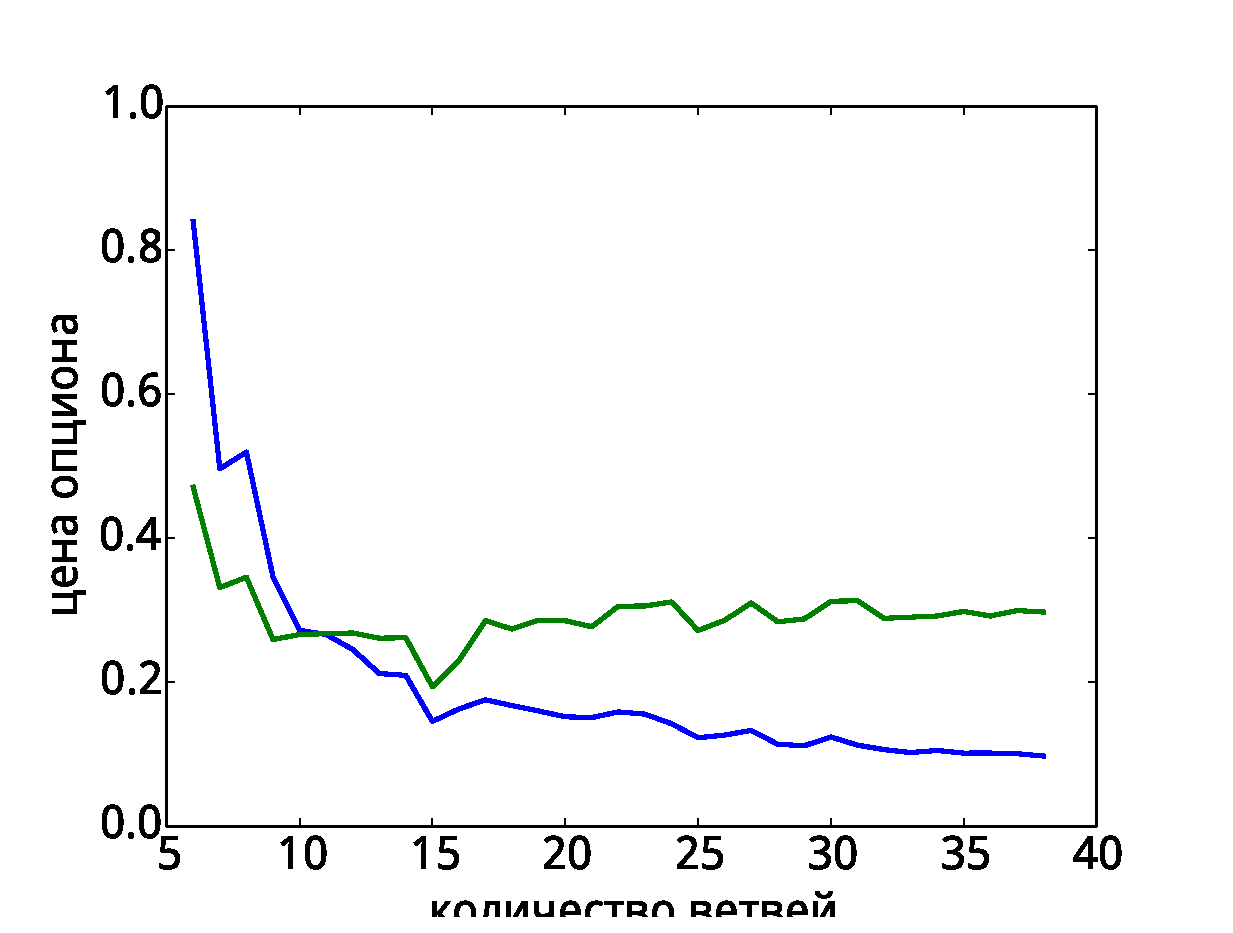
\includegraphics[width=0.8\textwidth]{true_value_test_empiric_distr}
    		\caption{Верхняя и нижняя оценки стоимости опциона по дереву с анализом эмпирической функцией распределения}
    		\label{fig:true_value_test_empiric_distr}
    		\footnotesize{Оценки стоимости опциона с начальной ценой 100, выписанного на срок 1 год на базовый актив с риск-нейтральной процентной ставкой $r = 0.05$, дивидендной ставкой $\delta = 0.1$ и волатильностью $\sigma=0.2$, цена которого --- случайный процесс, являющийся геометрическим броуновским движением с параметрами $\mu = r - \delta$ и $\sigma$, исполняемого 4 раза в году}
	    \end{figure}
		Из графика видно, что сходимости к истинному значению не наблюдается.
\section{Конечная сетка состояний}
	    \subsection{Описание метода}
	        Для того, чтобы сложность алгоритма по  памяти составляла $O(bm)$, необходимо начиная с некоторого момента ограничивать множество состояний, в которые может перейти актив из данного. Так как мы имеем дело с нестационарным случайным процессом, распределение состояний на следующем шаге меняется, как только мы получаем новую реализацию состояния на предыдущем шаге.

	        Можно использовать знания о законе распределения, которому подчиняется состояние базового актива, чтобы уменьшить число возможных состояний.
	        $$dS_t = \mu S_t dt + \sigma S_t dW_t \implies \log \left(\frac{S_t}{S_0}\right)\sim N\left(\left(\mu - \frac{\sigma^2}{2}\right)t, \sigma^2 t\right).$$
	        Ограничив множество состояний базового актива в момент времени $t$ числом $n$, мы можем рассчитать, попадание в какие $n$ классов состояний будет равновероятно. Пусть $F(x)$ --- функция распределения $N\left(0, 1\right)$, тогда
	        \begin{align}
	            \forall i \in 1:n \;\;\exists\; \xi_i = F^{-1}\left(\frac{i-0.5}{n}\right) \text{ --- представитель $i$-го состояния} ,\\
	            \forall i \in 0:n \;\;\exists\; z_i = F^{-1}\left(\frac{i}{n}\right) \text{ --- граница $i$-го состояния} .
	        \end{align}
	        Для каждого момента времени $t_i$ определено множество состояний $$S_i^j = S_0\exp\left(\left(\mu - \frac{\sigma^2}{2}\right)t + \sigma \sqrt{t}\xi_j\right), j\in 1:n$$ и множество границ этих состояний $$Z_i^j = S_0\exp\left(\left(\mu - \frac{\sigma^2}{2}\right)t + \sigma \sqrt{t}z_j\right), j\in 1:n.$$
	        Для любого состояния $S_i^{j_1\cdots j_i}$ найдётся $k\in 1:n : Z_i^{k-1} \leq S_i^{j_1\cdots j_i} < Z_i^k$, тогда $S_i^{j_1\cdots j_i} := S_i^j$.
	        Множество состояний не зависит от имеющихся результатов моделирования, только от параметров базового актива, следовательно, генерируемые траектории будут достаточно независимы, чтобы подходить под условия сходимости оценок \eqref{eq:upper-terminal}-\eqref{eq:upper-node}, \eqref{eq:lower-terminal}-\eqref{eq:lower-node}. Количество возможных состояний на каждом шаге можно увеличивать по мере увеличения $t_i$, что может частично компенсировать растущую дисперсию.
	        \subsection{Численные результаты}
	            Результаты моделирования для оценки стоимости того же опциона, что был использован для демонстрации классического алгоритма, представлены на рис. \ref{fig:true_value_test_finite_grid}
                \begin{figure}[h]
                    \centering
                    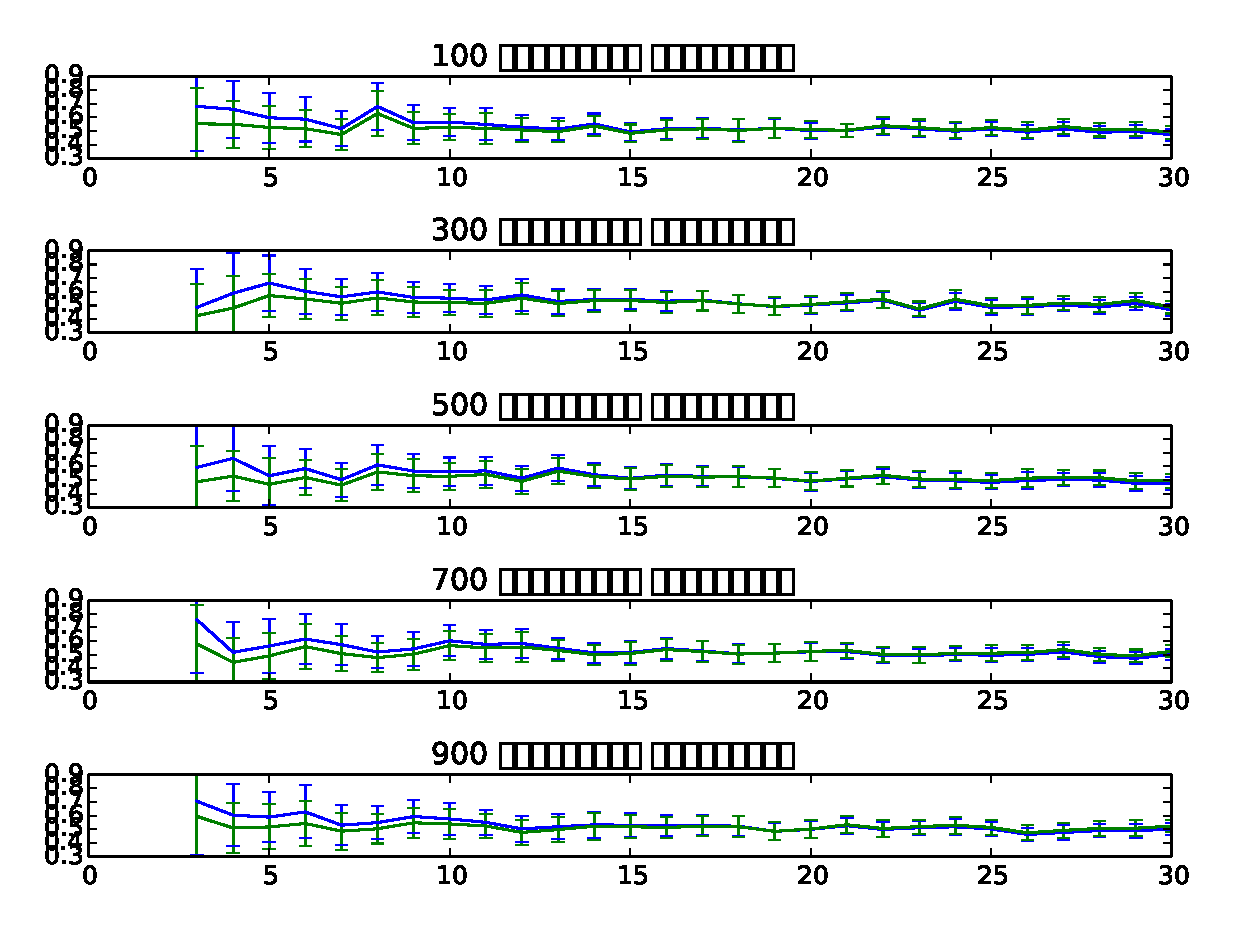
\includegraphics[width=\textwidth]{true_value_test_finite_grid}
                    \caption{Верхняя и нижняя оценки стоимости опциона по дереву с анализом эмпирической функцией распределения}
                    \label{fig:true_value_test_finite_grid}
                    \footnotesize{Оценки стоимости опциона с начальной ценой 100, выписанного на срок 1 год на базовый актив с риск-нейтральной процентной ставкой $r = 0.05$, дивидендной ставкой $\delta = 0.1$ и волатильностью $\sigma=0.2$, цена которого --- случайный процесс, являющийся геометрическим броуновским движением с параметрами $\mu = r - \delta$ и $\sigma$, исполняемого 4 раза в году}
                \end{figure}
                Несмотря на выполнение условий сходимости, налагаемых на траектории, вычисления демонстрируют отсутствие сходимости при $b \to \infty$: при больших значениях $b$ ($b=60, 80$, не показаны на графике) оценки демонстрируют устойчивое поведение, и среднее значение верхней и нижней оценки по 100 реализаций для каждого $b$ равны $0.48\pm 0.02$ и $0.43\pm 0.03$ соответственно.